\documentclass[10pt,a4paper]{article}

\usepackage[utf8]{inputenc}
\usepackage[T1]{fontenc}
\usepackage[english]{babel}
\usepackage{lmodern}
\usepackage[a4paper,margin=20mm,includeheadfoot,headheight=20pt,headsep=6mm,footskip=10mm]{geometry}
\usepackage{amsmath,amssymb}
\usepackage{graphicx}
\usepackage{xcolor}
\usepackage{fancyhdr}
\usepackage[hidelinks]{hyperref}

\setlength{\parindent}{0pt}
\setlength{\parskip}{3pt}

\newcommand{\StudentNames}{Aurian Borzée (s224392), Angélique Fontenelle (s2301647), Thomas Noël (S194057)}

\newif\ifmainreport
\mainreporttrue
\newcounter{MainReportPages}
\newcommand{\EndMainReport}{%
  \clearpage
  \setcounter{MainReportPages}{\numexpr\value{page}-1\relax}%
  \mainreportfalse
  \ifnum\value{MainReportPages}>4\relax
    \PackageWarningNoLine{elen0062-report}{MAIN REPORT EXCEEDS FOUR PAGES:
      \arabic{MainReportPages} counted pages. The AI-use
      declaration is excluded. Shorten the main report}%
  \fi
  {\small This page does not count toward the 4-page limit.\par}\medskip
}
\AtEndDocument{%
  \ifmainreport
    \PackageWarningNoLine{elen0062-report}{The required EndMainReport marker
      is missing. The main-report page count cannot be confirmed}%
  \fi
}

\pagestyle{fancy}
\fancyhf{}
\fancyhead[L]{%
  \ifmainreport
    \ifnum\value{page}>4\relax
      \Large\color{red!65!black}\textbf{MAIN REPORT EXCEEDS FOUR PAGES}%
    \else
      \small ELEN0062 -- Project 1%
    \fi
  \else
    \small ELEN0062 -- Project 1%
  \fi
}
\fancyhead[R]{%
  \ifmainreport
    \ifnum\value{page}>4\relax
    \else
      \small 2026--2027%
    \fi
  \else
    \small 2026--2027%
  \fi
}
\fancyfoot[R]{\ifmainreport\small\thepage\fi}
\renewcommand{\headrulewidth}{0.3pt}
\renewcommand{\footrulewidth}{0pt}


% ---- Figure helpers ----
\graphicspath{{../code/output_dt/}{../code/output_knn/}{../code/output_nb/}{../code/output_mc/}}

\newcommand{\cell}[1]{%
  \begin{minipage}[c]{0.30\textwidth}
    \centering
    #1
  \end{minipage}%
}

\newcommand{\fg}[1]{%
  \includegraphics[width=\linewidth]{#1}%
}

\newcommand{\fgx}[1]{%
  \includegraphics[width=\linewidth]{#1}%
}

\newcommand{\tab}[2]{%
  \begin{minipage}[c]{\linewidth}
    \centering
    \scriptsize
    \begin{tabular}{lc}
      \multicolumn{2}{c}{#1}\\
      \hline
      #2
    \end{tabular}
  \end{minipage}%
}

\begin{document}

\begin{center}
  {\large\bfseries Project 1 -- Classification algorithms}\par
  {\small\StudentNames}
\end{center}

\section{Decision tree}
\subsection{Decision boundaries and model complexity}



\begin{figure}[!htb]
\centering
\begin{tabular}{ccc}
  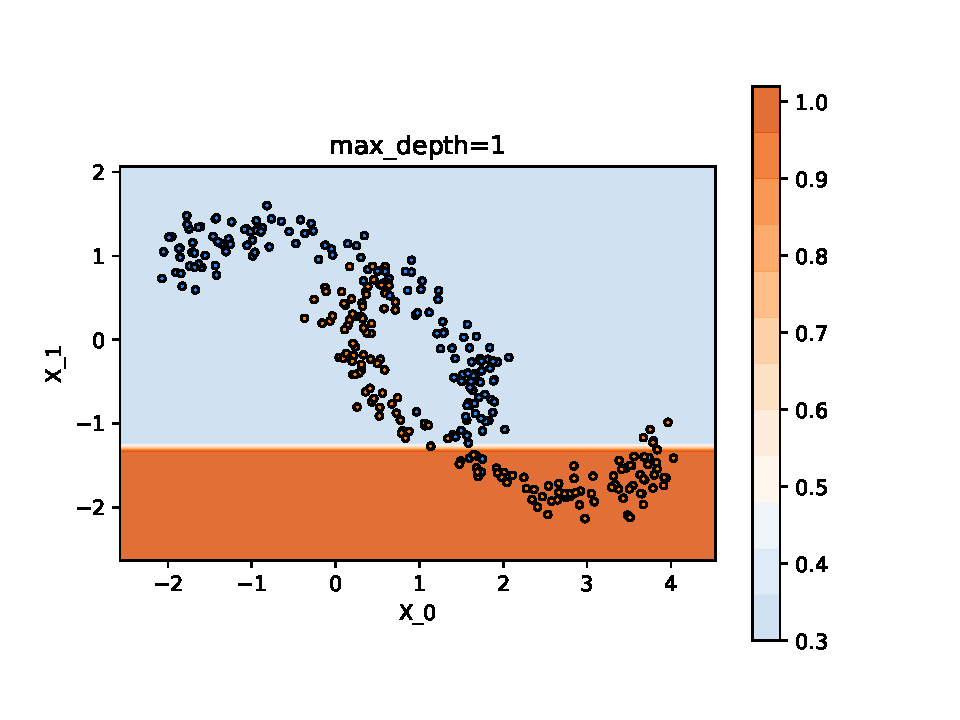
\includegraphics[width=0.30\textwidth,trim=18pt 30pt 62pt 34pt,clip]{dt_depth_1.pdf} &
  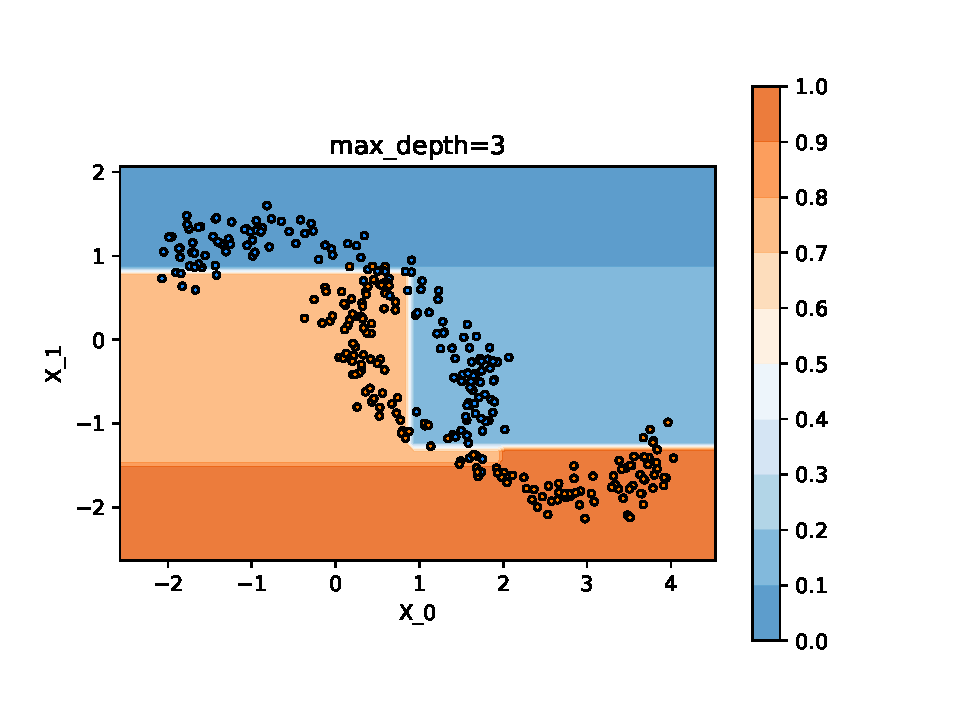
\includegraphics[width=0.30\textwidth,trim=18pt 30pt 62pt 34pt,clip]{dt_depth_3.pdf} &
  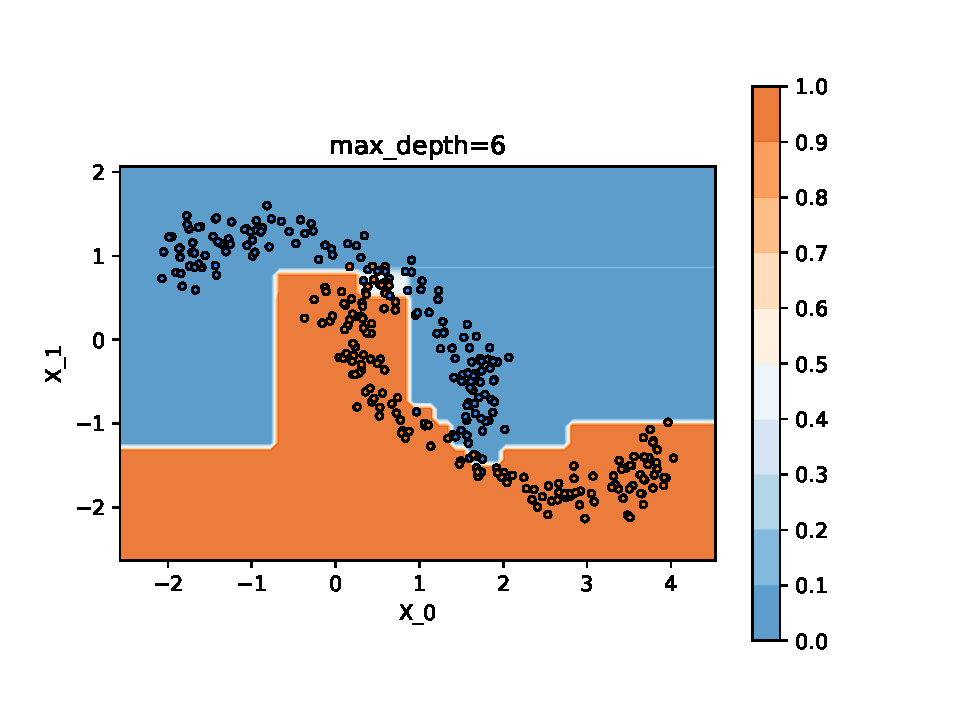
\includegraphics[width=0.30\textwidth,trim=18pt 30pt 62pt 34pt,clip]{dt_depth_6.pdf} \\
  [4pt]
  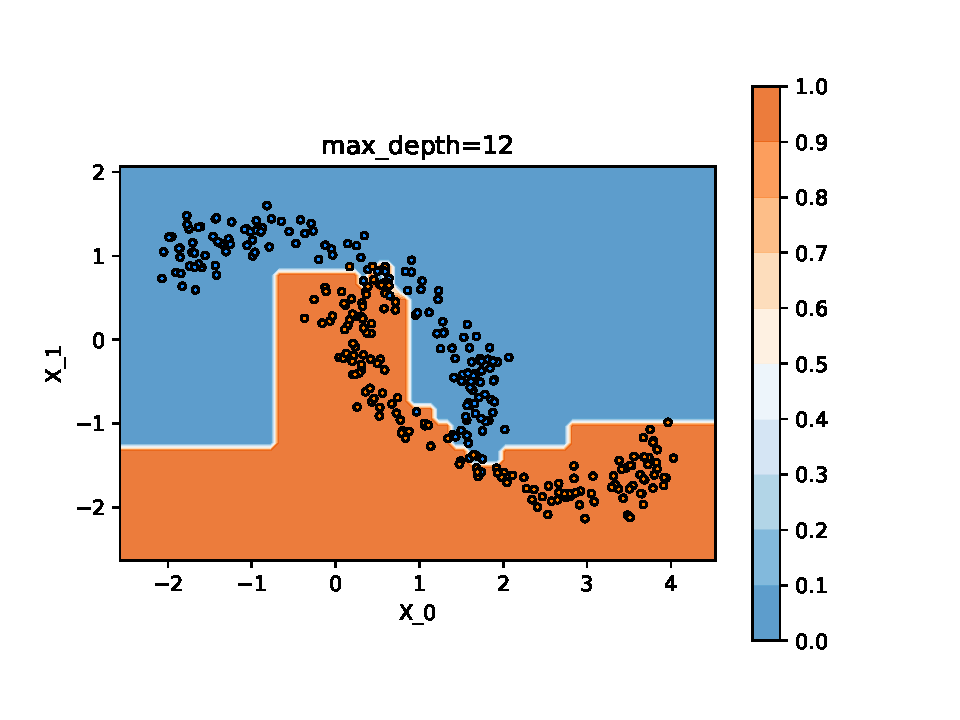
\includegraphics[width=0.30\textwidth,trim=18pt 30pt 62pt 34pt,clip]{dt_depth_12.pdf} &
  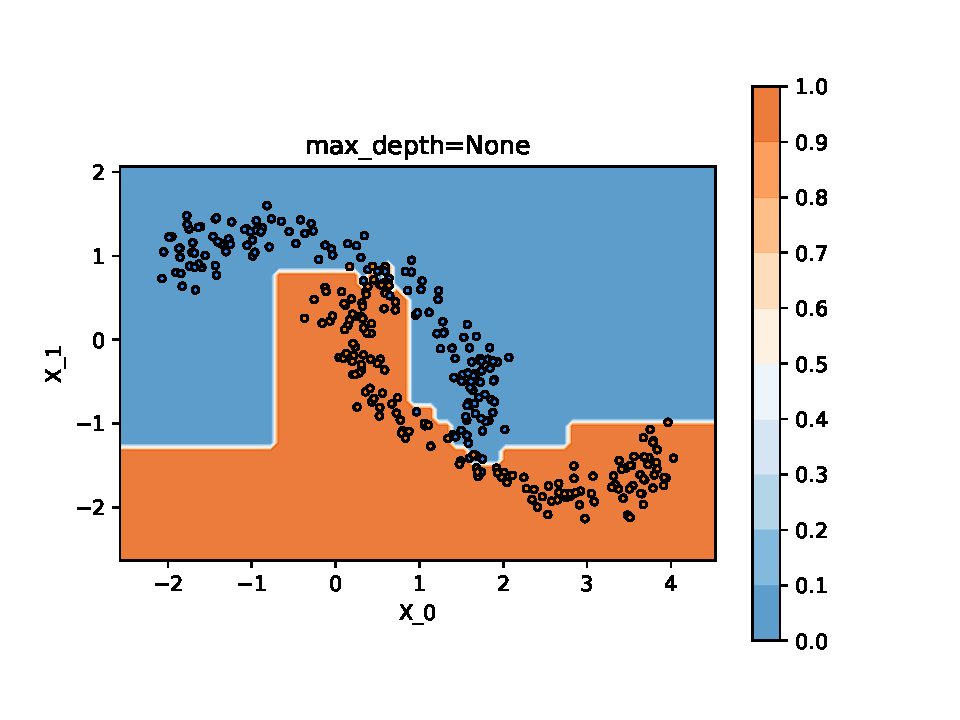
\includegraphics[width=0.30\textwidth,trim=18pt 30pt 62pt 34pt,clip]{dt_depth_None.pdf} &
  \begin{minipage}[c]{0.30\textwidth}
    \centering
    \scriptsize
    \begin{tabular}{lc}
      \multicolumn{2}{c}{\textbf{Test accuracy}}\\
      \multicolumn{2}{c}{\textbf{(5 generations)}}\\
      \hline
      Depth & Mean $\pm$ std\\
      \hline
      1    & $0.731 \pm 0.015$\\
      3    & $0.887 \pm 0.019$\\
      6    & $0.951 \pm 0.010$\\
      12   & $0.950 \pm 0.020$\\
      None & $0.949 \pm 0.020$\\
      \hline
    \end{tabular}
  \end{minipage}
\end{tabular}
\caption{Decision tree. Boundaries: seed 0, 1200/300 learning/test points, drawn on the test points (background: $P(y{=}1|x)$). Table: seeds 0--4.}
\label{fig:dt}
\end{figure}



\textbf{(a)} A tree only makes axis-aligned splits, so each boundary is a union of rectangles. Depth 1: one split. Depth 3 (7 leaves): a coarse staircase. Depth 6 (28 leaves): the moons are followed. Depth 12 and \texttt{None} (54, 56 leaves): small rectangles isolate single points. The moons are oblique, hence the many leaves needed.

\textbf{(b)} \emph{Underfitting}: depths 1 and 3, with low accuracy on both sets (train/test 0.748/0.713 and 0.877/0.900), i.e.\ a bias error. \emph{Overfitting}: depth 12 and \texttt{None} reach 0.998 and 1.000 on the learning set but their test accuracy (0.960, 0.957) is no better than depth 6 (0.950); the train--test gap grows from 0.024 (depth 6) to 0.038 and 0.043 as rectangles fit noisy points. Depth 6 is the best compromise.

\textbf{(c)} Deeper trees have purer leaves: the mean $\max_y P(y|x)$ on the test points is 0.745, 0.872, 0.971, 0.999, 1.000. At maximal depth each leaf holds one class, so \texttt{predict\_proba} is 0 or 1 almost everywhere: this confidence reflects memorisation of the learning set (variance), not reliability.

\subsection{Accuracy over five generations}
Accuracy rises up to depth 6 (0.731, 0.887, 0.951), then stagnates (0.950, 0.949); the std doubles for depth 12 and \texttt{None} (0.020 vs 0.010): deep trees are less stable. Depth 6 has the best mean and the lowest variance.

\section{K-nearest neighbors}
\subsection{Decision boundaries and number of neighbors}

\begin{figure}[!htb]
\centering
\cell{\fg{knn_1.pdf}}\hfill\cell{\fg{knn_9.pdf}}\hfill\cell{\fg{knn_45.pdf}}\par\smallskip
\cell{\fg{knn_225.pdf}}\hfill\cell{\fg{knn_901.pdf}}\hfill
\cell{\tab{\texttt{n\_neighbors}}{
  1   & $0.947 \pm 0.015$\\
  9   & $0.959 \pm 0.012$\\
  45  & $0.958 \pm 0.011$\\
  225 & $0.953 \pm 0.011$\\
  901 & $0.619 \pm 0.021$\\
}}
\caption{K-nearest neighbors: boundaries (seed 0) and accuracy over seeds 0--4.}
\label{fig:knn}
\end{figure}

\textbf{(b)} For $k{=}1$ the boundary is irregular: each learning point owns a region (train 1.000, test 0.953) and noisy points make it jagged (high variance). For $k{=}9$ and $45$ it is smooth and follows the moons (test 0.950, 0.953). For $k{=}225$ the boundary is very smooth and the probabilities become blurred near the moons (0.947/0.947). For $k{=}901$ (three quarters of the learning set) each prediction averages most of the data: the boundary is almost a straight line and the probabilities stay in about $[0.35, 0.65]$: underfitting (0.657/0.587).

\subsection{Accuracy over five generations}
Accuracy is almost constant for $k$ from 9 to 225 (0.953--0.959, within one std) and collapses for $k{=}901$ (0.619). $k{=}1$ is slightly worse (0.947, std 0.015) because of its variance.

\section{KDE Naive Bayes}
\subsection{Equivalence of (3) and (1)}
By Bayes' rule $p(y|x)=p(y)\,p(x|y)/p(x)$ and $p(x)$ does not depend on $y$, so $\operatorname{argmax}_y p(y|x)=\operatorname{argmax}_y p(y)\,p(x_1,\dots,x_p|y)$. By the chain rule $p(x_1,\dots,x_p|y)=\prod_{i}p(x_i|y,x_1,\dots,x_{i-1})$ and by (2), with $Z=\{X_1,\dots,X_{i-1}\}$, each factor equals $p(x_i|y)$. This gives (3).

\subsection{Implementation}
\texttt{fit} stores the sorted classes, the priors (class ratios) and the learning points of each class, which define the 1D Gaussian KDEs (4)--(5). We compute $\log p(y)+\sum_i\log\hat p(x_i|y)$, each KDE term with a log-sum-exp over the learning points (kernels underflow for small $h$), and normalise the posterior with a log-sum-exp over the classes. The result matches scikit-learn's \texttt{KernelDensity}.

\subsection{Effect of the bandwidth}

\begin{figure}[!htb]
\centering
\cell{\fg{nb_h0.005.pdf}}\hfill\cell{\fg{nb_h0.03.pdf}}\hfill\cell{\fg{nb_h0.2.pdf}}\par\smallskip
\cell{\fg{nb_h0.8.pdf}}\hfill\cell{\fg{nb_h3.2.pdf}}\hfill
\cell{\tab{$h$}{0.005 & $0.838 \pm 0.015$\\ 0.03 & $0.905 \pm 0.024$\\ 0.2 & $0.937 \pm 0.016$\\ 0.8 & $0.760 \pm 0.035$\\ 3.2 & $0.640 \pm 0.023$}}
\caption{KDE Naive Bayes: boundaries (seed 0) and accuracy over seeds 0--4.}
\label{fig:nb}
\end{figure}

For $h{=}0.005$ each 1D density is a spike on every learning value, so the posterior is an irregular grid-like pattern and the train accuracy (0.952) is far above the test one (0.860): overfitting. For $h{=}0.03$ the densities are smoother and both agree (0.922/0.920); $h{=}0.2$ is the best trade-off (0.934/0.943). For $h{=}0.8$ and $3.2$ the densities are over-smoothed and the classes get similar wide marginals: for $h{=}0.8$ the boundary is a wide smooth band that no longer follows the shape of the moons, and for $h{=}3.2$ it is almost a straight line with a posterior within about $[0.3,0.7]$: underfitting (0.769/0.733, then 0.676/0.603).

\subsection{Accuracy over five generations}
The accuracy peaks at $h{=}0.2$ (0.937), is lower for $h{=}0.03$ (0.905) and $0.005$ (0.838, variance) and drops for large $h$ (0.760, 0.640); the std is largest at the extremes (up to 0.035). Even at its best $h$, NB stays below the tree and KNN (0.95--0.96), see Section~4.

\section{Method comparison}
\subsection{Tuning protocol}
The candidates are the values above. We use a stratified 5-fold cross-validation \emph{on the learning set only}: each value is trained on 4 folds and scored on the held-out one, the best mean accuracy is kept and the model is refitted on the whole learning set; the test set is only used at the end. Each fold trains on 960 points, so $k{=}901$ remains possible (a 75/25 hold-out leaves 900 points, fewer than $k$).

\subsection{Accuracy on the two-moon dataset}

\begin{figure}[!htb]
\centering
\cell{\fg{moons_decision_tree.pdf}}\hfill\cell{\fg{moons_knn.pdf}}\hfill\cell{\fg{moons_kde_naive_bayes.pdf}}\par\smallskip
\cell{\fgx{xor_decision_tree.pdf}}\hfill\cell{\fgx{xor_knn.pdf}}\hfill\cell{\fgx{xor_kde_naive_bayes.pdf}}
\caption{Tuned models (seed 0, test points). Top: two moons. Bottom: XOR.}
\label{fig:mc}
\end{figure}



Mean test accuracy $\pm$ std over seeds 0--4: \textbf{decision tree $0.954\pm0.013$}, \textbf{KNN $0.960\pm0.012$}, \textbf{KDE Naive Bayes $0.937\pm0.016$}. Selected values: depth 6 (three times) or 12, $k{=}9$ (four times) or 45, $h{=}0.2$ every time.

\subsection{Ranking on the two moons}
KNN $\geq$ tree $>$ KDE Naive Bayes. KNN and the tree differ by less than one std, so five generations cannot separate them; NB is about two points below. KNN and the tree make no assumption on how $X_0$ and $X_1$ depend on each other: KNN follows the moons smoothly, the tree with a staircase. NB assumes that $X_0$ and $X_1$ are independent given the class, which is false here (each class is a curved arc, so $X_1$ depends strongly on $X_0$): the product of marginals captures the dense core of each moon but not the crescents, and outside the data its boundary is a large oblique wedge (Fig.~\ref{fig:mc}, top right).

\subsection{XOR dataset}
On XOR (Fig.~\ref{fig:mc}, bottom) the means $\pm$ std are: \textbf{tree $1.000\pm0.000$} (depth 6 four times, 3 once), \textbf{KNN $0.978\pm0.008$}, \textbf{NB $0.507\pm0.030$}, i.e.\ chance. The bandwidth selected for NB varies a lot (0.03, 0.2 or 3.2) because no value helps.

\subsection{Comparison on XOR}
XOR is exactly two axis-aligned splits ($x_0{=}0$, $x_1{=}0$), so the tree is perfect. KNN is local and also fits it, its few errors lying near the axes where the quadrants meet. NB fails by construction: in each class the marginals of $X_0$ and $X_1$ are the same uniform density on $[-2,2]$ (each sign is equally likely in both classes), so each factor $p(x_i|y)$ in (3) is the same for both classes and the posterior reduces to the prior (0.5); the faint stripes of its map (probabilities 0.36--0.69) are noise. The label depends on the \emph{joint} behaviour of $X_0$ and $X_1$ (sign of $x_0x_1$), which assumption (2) removes. The KDE models complex 1D densities well, but here the marginals carry no information on $y$: the failure comes from the factorisation, not from the density estimator.

% All report content must stay above this marker.
\EndMainReport

\section*{AI-use declaration}

Several AI tools were used during the development of this project:
\textbf{Claude, Gemini, and ChatGPT (GPT)}. The tools were selected
according to their respective strengths and usefulness for specific tasks.

AI assistance was used for the following purposes:

\begin{itemize}
  \item \textbf{Utility code:} AI was used to assist with the development
  of the \texttt{utils.py} file.

  \item \textbf{Terminal output presentation:} AI helped format and
  organize terminal outputs to make them clearer and more readable.

  \item \textbf{Report writing:} AI assisted with the drafting,
  structuring, and LaTeX formatting of parts of the report.

  \item \textbf{Code review:} AI tools were used to review the code,
  identify potential issues, and suggest improvements.
\end{itemize}

The overall code organization, project architecture, and core
implementation were designed and developed by the team members.
AI tools were used as supporting tools rather than as substitutes
for the team's own work.

AI-generated suggestions were reviewed by the team and checked
against the project's requirements and expected behavior.
Code-related suggestions were assessed for correctness and consistency
with the existing implementation, while report content and formatting
were reviewed before inclusion. The team remains responsible for
the final code, results, and report.


\end{document}